\section{Introduction}

Large language models are increasingly used as research assistants: they summarize papers, draft reviews, suggest experiments, and help authors revise manuscripts.
For these systems, static critique is not enough.
A scientifically useful assistant must update its judgment when the paper changes.
If a reviewer originally asked for computational-cost evidence and the revision adds a direct cost comparison, then repeating the old criticism is no longer helpful.
Conversely, a long and polite author response does not mean the concern was actually fixed.

\begin{figure*}[t]
\centering
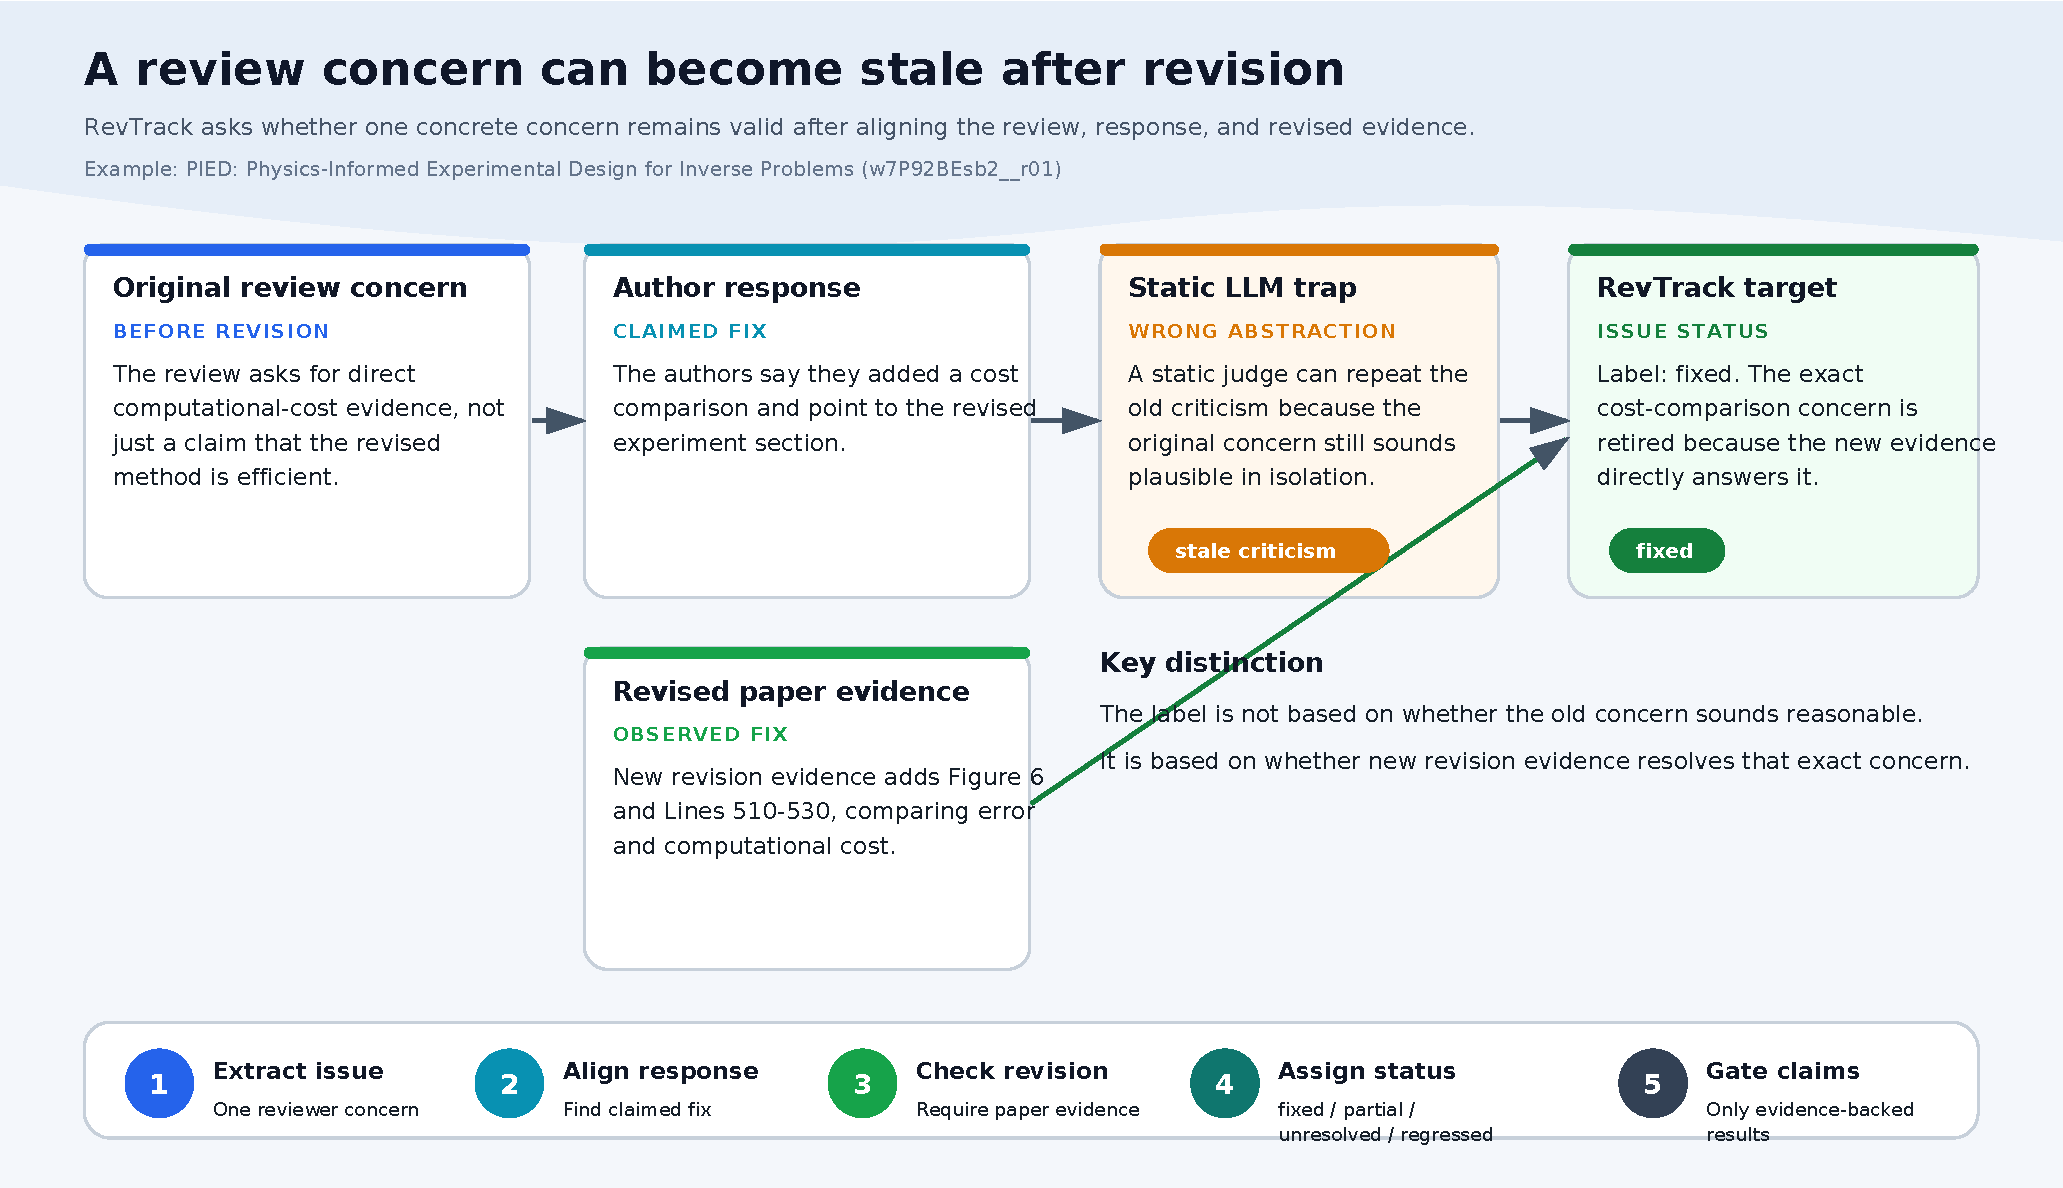
\includegraphics[width=\textwidth]{figures/figure1_revision_tracking.pdf}
\caption{RevTrack exposes a temporal failure mode: a criticism that is valid before revision can become stale after new evidence is added. The benchmark aligns each concern to the author response and revised-paper evidence before assigning an issue status, preventing static assistants from repeating obsolete criticism.}
\label{fig:running-example}
\end{figure*}

This paper studies revision-status tracking: given a paper context, one reviewer concern, author response evidence, and a revision summary, predict whether the original concern is \textit{fixed}, \textit{partially fixed}, \textit{unresolved}, or \textit{regressed}.
The task targets an evaluation blind spot.
Many review-assistance evaluations ask whether a model can produce plausible critiques, answer reviewer questions, or rate paper quality.
Those settings do not measure whether the model can maintain a structured memory of scientific concerns across revision.
As a result, systems can appear competent while still failing at the workflow that matters to authors, reviewers, and program chairs: deciding which concerns remain unresolved after the evidence changes.

We introduce \textsc{RevTrack}, a benchmark and diagnostic suite for revision-aware scientific judgment.
RevTrack builds issue-level examples from public OpenReview discussions, prioritizes hard cases with model disagreement, and keeps blind validation sheets separate from assistant/model keys.
The benchmark is organized around evidence rather than surface plausibility: each label must be supported by a review concern span, a response or revision evidence span, and a short boundary note.
The current standard validation set covers 301 audit rows across ICLR 2024, ICLR 2025, NeurIPS 2024, and ICLR 2023.
It includes 80-row active frontiers for ICLR 2025 and NeurIPS 2024, plus an 80-row ICLR 2023 random/stratified slice; all standard rows have complete evidence spans.

The empirical picture is deliberately diagnostic rather than model-chasing.
On the hardened ICLR 2024 clean-dev benchmark, a structured evidence model reaches 0.704 macro-F1, compared with 0.389 for the strongest semantic encoder baseline.
At the same time, cross-year transfer exposes brittleness.
On the ICLR 2025 stress set, a TF-IDF model matches the majority baseline in accuracy while assigning zero F1 to fixed cases.
On the standard-labeled expanded80 frontier, the best model reaches only 0.469 macro-F1; structured transfer over-credits unresolved concerns in 66 cases, while TF-IDF misses all fixed and regressed examples in that frontier.
On the user-confirmed NeurIPS 2024 active frontier, the best transferred semantic encoder reaches 0.348 macro-F1, while prompted LLMs and calibrated votes remain near the majority reference.
The ICLR 2023 random/stratified slice adds bounded external-validity evidence outside disagreement-focused active frontiers while preserving the same no-IAA and no-natural-prevalence boundary.

The central contribution is therefore not a new state-of-the-art review model.
\textsc{RevTrack} argues that the community is measuring the wrong capability for scientific assistants.
A useful assistant must not merely produce a plausible static review; it must track evidence over time, retire stale criticism, resist superficial reassurance, and flag regressions when revision makes a concern worse.
To make these claims auditable, the release includes packet-integrity checks, leakage controls, label-evidence audits, a failure taxonomy, and a claim ledger that blocks overclaiming.

Our contributions are:
\begin{itemize}[leftmargin=*]
\item We define revision-status tracking as an issue-level task for scientific review assistance.
\item We release a reproducible construction and validation pipeline with blind/key separation, evidence-span auditing, leakage checks, and claim-readiness gates.
\item We provide a validated ICLR 2024 benchmark slice, a 21-row ICLR 2025 stress set, 80-row user-confirmed active frontiers for ICLR 2025 and NeurIPS 2024, and an 80-row ICLR 2023 random/stratified standard slice.
\item We show that semantic baselines can look reasonable by accuracy while failing fixed, unresolved, and regressed-case recovery.
\item We demonstrate that structured revision evidence improves in-domain macro-F1 and use prompted LLMs, vote ensembles, and a failure taxonomy to explain where transfer models still break.
\end{itemize}
